\documentclass[12pt]{article}
\usepackage[english]{babel}
\usepackage[letterpaper,top=2cm,bottom=2cm,left=3cm,right=3cm,marginparwidth=1.75cm]{geometry}
\usepackage{amsmath}
\usepackage{amsfonts}
\usepackage{graphicx}
\usepackage{float}
\DeclareMathOperator{\pv}{pv}
\DeclareMathOperator{\pva}{pva}
\renewcommand{\theenumi}{\alph{enumi}}
\makeatletter
\renewcommand{\thesection}{Part \Roman{section}}
\renewcommand{\thesubsection}{\arabic{subsection}}
\makeatother
\title{FINC-UB 2 Homework 4}
\author{Ishan Pranav}
\date{September 20, 2023}
\begin{document}
\maketitle
\section{Constructing portfolios}
\subsection{Suppose you want to use your savings accounts to build a portfolio}
\begin{enumerate}
\item The investor's equity is $\$1000$. $\$1000=\$500+\$400+\$700-x$, where $x$ is the liability associated with the short position in Twitter. Then $x=\$600$.
\begin{center}
\begin{tabular}{l|cr|r}
\textbf{Security}&&\textbf{Investment}&\textbf{Weight}\\
Google&\$&500&0.5\\
Apple&\$&400&0.4\\
Amazon&\$&700&0.7\\
Twitter&(\$&600)&-0.6\\
\textbf{Total}&\textbf{\$}&\textbf{1000}&\textbf{1.0}\\
\end{tabular}
\end{center}
\item As demonstrated above, the value of the short position in Twitter is \$600.
\item The amount invested in Google and Apple does not change. Amazon remains a long position, and Twitter remains a short position with \$250 invested (short).
\begin{center}
\begin{tabular}{l|cr|r}
\textbf{Security}&&\textbf{Investment}&\textbf{Weight}\\
Google&\$&500&0.50\\
Apple&\$&400&0.40\\
Amazon&\$&350&0.35\\
Twitter&(\$&250)&-0.25\\
\textbf{Total}&\textbf{\$}&\textbf{1000}&\textbf{1.00}\\
\end{tabular}
\end{center}
\end{enumerate}
\subsection{Securities \textit{A} and \textit{B}}
\begin{enumerate}
\item The investment opportunity set is depicted in Figure~\ref{fig:ios}. The efficient frontier is the upward-sloping part of the hyperbola; that is, the subset of all portfolios with an expected return greater than approximately 14.16\%.
\item Let $\sigma_p$ be the standard deviation of the portfolio.

\begin{align*}
\sigma_p^2
&=w_A^2\sigma_A^2+w_B^2\sigma_B^2+2w_Aw_B\rho_{A,B}\sigma_A\sigma_B\\
&=\left(15.4\%^2\times w_A^2\right)+\left(23.0\%^2\times w_B^2\right)+2w_Aw_B(-1)(15.4\%)(23.0\%)\\
&=\left(15.4\%^2\times w_A^2\right)+\left(23.0\%^2\times w_B^2\right)-(7.084\%\times w_Aw_B)\\
0&=\left(15.4\%^2\times w_A^2\right)+\left(23.0\%^2\times(1-w_A)^2\right)-(7.084\%\times w_A(1-w_A)))\\
w_A&\approx 0.5990\dots
\end{align*}

Then $w_B=1-w_A\approx 0.4010\dots$

\item The expected return of the risk-free portfolio is approximately 14.16\%.
\item The only risk-free rate consistent with no-arbitrage is approximately 14.16\%. All risk-free securities are indistinguishable from the one we constructed. Therefore, market forces price all risk-free securities to yield the same return (supply and demand with perfect substitutes).
\begin{figure}
\begin{center}
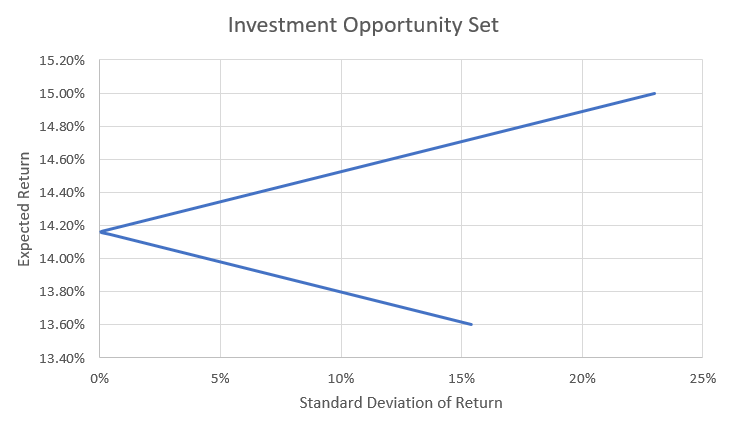
\includegraphics[width=4in]{images/ios.png}
\end{center}
\caption{The investment opportunity set of portfolios containing $A$ and $B$.\label{fig:ios}}
\end{figure}
\end{enumerate}
\section{Ordinary least squares mechanics}
\subsection{Prove that the mean residual is 0}
Let $\hat{\epsilon}_i$ be the residual from $i=1$ to $N$ observations. We want to show that the mean residual is 0. Observe
\begin{align*}
\hat{\epsilon}_i&=y_i-\hat{y}_i&\textit{predicted residual}\\
\frac{1}{N}\sum_{i=1}^N{\hat{\epsilon}_i}&=\frac{1}{N}\sum_{i=1}^N{(y_i-\hat{y}_i)}.&\textit{mean predicted residual}
\end{align*}

Let $\hat{\beta}_0$ be the predicted constant coefficient and $\hat{\beta}_1$ be the predicted linear coefficient.

\begin{align*}
\frac{1}{N}\sum_{i=1}^N{\hat{\epsilon}_i}
&=\frac{1}{N}\sum_{i=1}^N{\left(y_i-(\hat{\beta_0}+\hat{\beta_1}x_i)\right)}&\textit{predicted least-squares regression equation}\\
&=\frac{1}{N}\sum_{i=1}^N{(y_i-\hat{\beta_0}-\hat{\beta_1}x_i)}.&\textit{distributive property of negation}
\end{align*}

Let $\bar{y}$ be the sample mean of all $y_i$ values and $\bar{x}$ be the sample mean of all $x_i$ values. Note $i=1$ to $N$.

\begin{align*}
\frac{1}{N}\sum_{i=1}^N{\hat{\epsilon}_i}
&=\frac{1}{N}\sum_{i=1}^N{\left(y_i-(\bar{y}-\hat{\beta_1}\bar{x})-\hat{\beta_1}x_i\right)}&\textit{predicted constant coefficient}\\
&=\frac{1}{N}\sum_{i=1}^N{(y_i-\bar{y}+\hat{\beta_1}\bar{x}-\hat{\beta_1}x_i)}&\textit{distributive property of negation}\\
&=\frac{1}{N}\left[\sum_{i=1}^N{y_i}-N\bar{y}+N\hat{\beta_1}\bar{x}-\hat{\beta_1}\sum_{i=1}^N{x_i}\right]&\textit{properties of summation}\\
&=\frac{1}{N}\sum_{i=1}^N{y_i}-\bar{y}+\hat{\beta_1}\bar{x}-\hat{\beta_1}\cdot\frac{1}{N}\sum_{i=1}^N{x_i}&\textit{distributive property of multiplication}\\
&=\bar{y}-\bar{y}+\hat{\beta_1}\bar{x}-\hat{\beta_1}\bar{x}&\textit{sample mean}\\
&=0.&\textit{arithmetic}
\end{align*}

We have shown that the expected value of the residual is 0.$~\square$
\subsection{Population parameters \textit{vs.} estimated coefficients}
The population parameters $\beta_0$ and $\beta_1$ model the true data points $y_i$ from $i=1$ to $N$. Since the actual data points do not fall exactly on a line, error terms ($\epsilon_i$) are introduced to offset each data point $(x_i,y_i)$ from the line given by $y_i=\beta_0+\beta_1x_i$. Meanwhile, $\hat{\beta_0}$ and $\hat{\beta_1}$ represent predictions for the line. These statistics estimate the line of best fit for the data points but cannot account for the errors. The statement $\hat{y}_i=\hat{\beta}_0+\hat{\beta}_1x_i$ would be interpreted ``on average, for each additional unit of $x_i$, the predicted score increases by $\hat{\beta_1}$. If $x_i=0$, the predicted score is $\hat{\beta}_0$.''
\subsection{$\hat{\beta}_1$ \textit{vs.} $\rho$}
The predicted linear coefficient $\hat{\beta}_1$ is interpreted: On average, for each additional unit of $x_i$, the predicted score increases by $\hat{\beta}_1$. The correlation coefficient $\rho$ indicates that as one variable changes in value, the other variable tends to change a specific direction as given by the sign of $\rho$.

The values of $\hat{\beta}_1$ and $\rho$ share the same sign, which indicates the direction of the relationship between the variables: 1 for a perfect positive relationship, -1 for a perfect inverse relationship, and 0 for no relationship whatsoever. Whereas $|\rho|$ provides the strength of the relationship, $\left|\hat{\beta}_1\right|$ provides the scale or amplification of the changes---the absolute slope of the regression line.
\subsection{The economic interpretation of $\hat{\beta}_0$}
In the Apple example, the economic interpretation of $\hat{\beta}_0=0.011011$ indicates that, according to the least-squares regression line, when the market (S\&P 500) excess return is 0\%, the predicted excess return of Apple is 1.1011\%.
\section{Running regressions}
\subsection{Describing the data}
Before computing monthly excess returns, we must convert the annual Fed funds rate and the annual risk-free rate to their effective monthly periodic equivalents. Then, for each security's monthly return, we subtract away the monthly risk-free rate.

\begin{figure}[h!]
\begin{center}
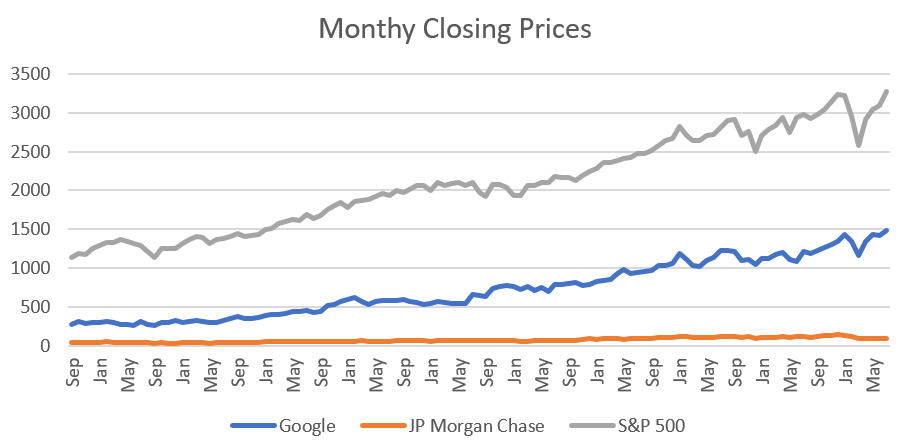
\includegraphics[width=4in]{images/monthly-closing-prices.png}
\end{center}
\caption{The monthly closing prices for Google, JP Morgan Chase, and the S\&P 500 index over time.\label{fig:monthly-closing-prices}}
\end{figure}
\begin{figure}[H]
\begin{center}
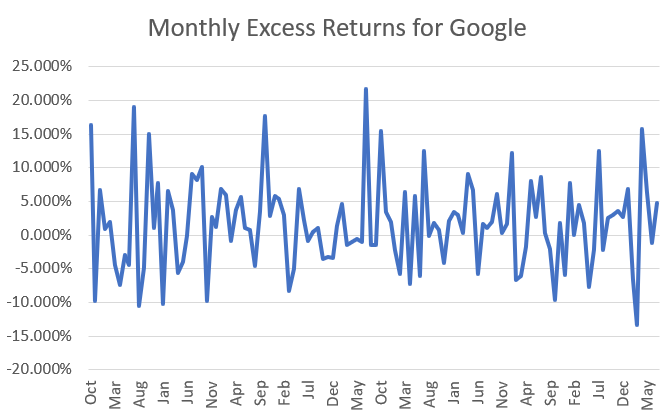
\includegraphics[width=4in]{images/google.png}
\end{center}
\caption{Google's excess returns above the effective risk-free rate for the one-month period over time.\label{fig:google}}
\end{figure}
\begin{figure}[H]
\begin{center}
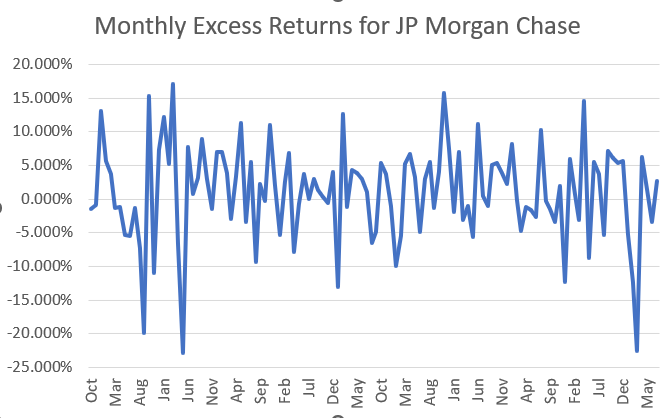
\includegraphics[width=4in]{images/jp-morgan-chase.png}
\end{center}
\caption{JP Morgan Chase's excess returns above the effective risk-free rate for the one-month period over time.\label{fig:jp-morgan-chase}}
\end{figure}
\begin{figure}[H]
\begin{center}
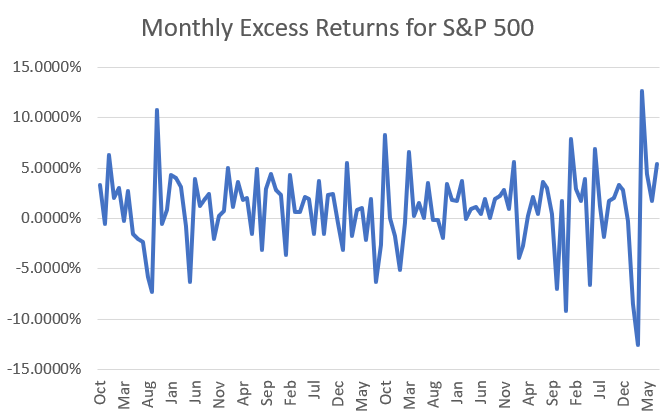
\includegraphics[width=4in]{images/spx.png}
\end{center}
\caption{The S\&P 500 index's excess returns above the effective risk-free rate for the one-month period over time.\label{fig:spx}}
\end{figure}
\subsection{Estimating regression models}
\begin{figure}[H]
\begin{center}
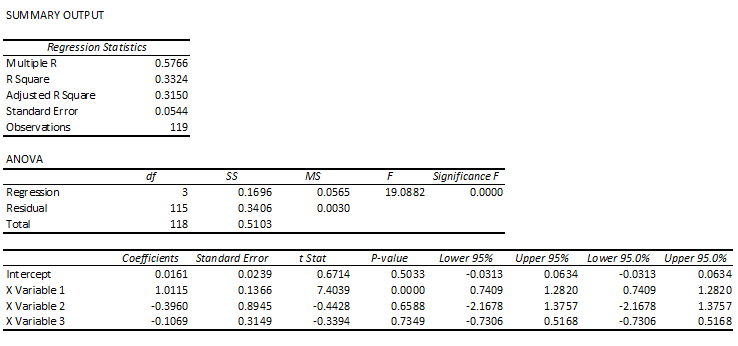
\includegraphics[width=6in]{images/google-regression.png}
\end{center}
\caption{Google's regression output.\label{fig:google-regression}}
\end{figure}
\begin{figure}[H]
\begin{center}
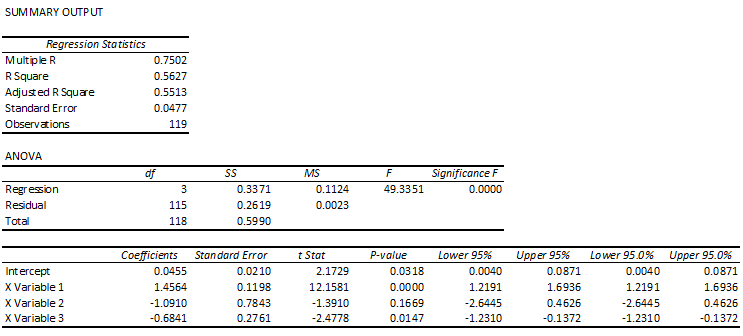
\includegraphics[width=6in]{images/jp-morgan-chase-regression.png}
\end{center}
\caption{JP Morgan Chase's regression output.\label{fig:jp-morgan-chase-regression}}
\end{figure}
\subsection{Interpreting regression results}
\begin{enumerate}
\item
\[H_0:\beta_1=\beta_2=\beta_3=0.\]
\[H_1:\beta_1\neq 0\text{ or }\beta_2\neq 0\text{ or }\beta_3\neq 0.\]

The null hypothesis is that S\&P 500 monthly excess returns, federal funds rate, and unemployment rate all have no significant relationship with the monthly excess returns of Google (or, in the second regression, JP Morgan Chase).
\item In both regressions, we can reject the null hypothesis for the S\&P 500 monthly excess returns. With respect to the excess returns of Google, the Student $t$-statistic for this independent variable is $t\approx 7.4039\dots$, and with respect to the excess returns of JP Morgan Chase, the Student $t$-statistic is $t\approx 12.1581\dots$ In both cases the $P$-value is significant ($P\approx 0.0000\dots$) at the $\alpha=0.0001$ significance level.

With respect to Google, the Student $t$-statistic for the Fed funds rate has $P\approx 0.6588\dots$, which is not significant at any common significance level (for example, not even $\alpha=0.1$). The Student $t$-statistic for the unemployment rate has $P\approx 0.7349\dots$, which is also not significant at any common significance level.

With respect to JP Morgan Chase, the Student $t$-statistic for the Fed funds rate has $P\approx 0.1669\dots$, which is not significant at any common significance level. The Student $t$-statistic for the unemployment rate has $P\approx 0.0147\dots$, which \textit{is} significant at the $\alpha=0.05$ and $\alpha=0.02$ significance levels, and other common significance levels more lenient than $\alpha=0.02$.

For Google, we reject $H_0$ because $\beta_1\neq 0$. For JP Morgan Chase, we reject $H_0$ because $\beta_1\neq 0$ and, depending on the significance level, $\beta_3\neq 0$. For all independent variables to be significant, the significance level would have to be at least $\alpha\approx 0.74\dots$
\item
$\beta_1\approx 1.0115\dots$: For each additional 1-percentage-point increase in the monthly excess return of the S\&P 500 index, the predicted monthly excess return of Google increases by approximately 1.01 percentage points.

$\beta_1\approx 0.3960\dots$: For each additional 1-percentage-point increase in the Fed funds rate, the predicted monthly excess return of Google decreases by approximately 0.396 percentage points.

$\beta_1\approx 0.1069\dots$: For each additional 1-percentage-point increase in the unemployment rate, the predicted monthly excess return of Google decreases by approximately 0.107 percentage points.
\newline

$\beta_1\approx 1.4564\dots$: For each additional 1-percentage-point increase in the monthly excess return of the S\&P 500 index, the predicted monthly excess return of JP Morgan Chase increases by approximately 1.46 percentage points.

$\beta_1\approx 1.0910\dots$: For each additional 1-percentage-point increase in the Fed funds rate, the predicted monthly excess return of JP Morgan Chase decreases by approximately 1.09 percentage points.

$\beta_1\approx 0.6841\dots$: For each additional 1-percentage-point increase in the unemployment rate, the predicted monthly excess return of JP Morgan Chase decreases by approximately 0.684 percentage points.
\item We use the coefficient of determination $r^2$ to determine the proportion of residuals captured by the ordinary least-squares regression line.

Approximately $r^2=33.24\%$ of the variation in the monthly excess returns of Google is explained by the variation in the monthly excess returns of the S\&P 500, the Fed fund, and the unemployment rate according to the least-squares regression line.

Approximately $r^2=56.27\%$ of the variation in the monthly excess returns of JP Morgan Chase is explained by the variation in the monthly excess returns of the S\&P 500, the Fed fund, and the unemployment rate according to the ordinary least-squares regression line.
\item There is a clear positive relationship between the monthly excess returns of Google and the S\&P 500 index \textit{and} between those of JP Morgan Chase and the S\&P 500 index. There may be an inverse relationship between the unemployment rate and the monthly excess returns of JP Morgan Chase, while the federal funds rate is neither clearly related to the monthly excess returns of Google nor to those of JP Morgan Chase.
\end{enumerate}
\end{document}